\chapter[Project Requirements]{Project Requirements}
\label{ch:reference}

\chapterepigraph{Rien n'est plus difficile, et donc plus pr\'ecieux, que d'\^etre capable de d\'ecider}{Napol\'eon Bonaparte}

\newthought{Here presented are the aims}, endpoints, controls, methods, schedule, and every relevant detail of the project; laid out unequivocally for reference before, during, and after the required work.

\section{Objectives and Deliverables}

\begin{margintable}
\vspace{12em}
\renewcommand{\arraystretch}{1.5}
\begin{tabular}
{p{8em} p{7em}}
		\toprule
		\emph{Deliverable} & \emph{Deadline} \\
		\midrule
		Prototype Game & Dec 6th 2012\\
		Progress Poster & Dec 6th 2012\\
		Final game & April 25th 2013\\
		Report & April 25th 2013\\
		Presentation & May 7th 2013 \\
		\bottomrule
\end{tabular}
\vspace{0.5em}
\caption{Summary of Deadlines}
\end{margintable}

The first objective of the project team is to produce a playable prototype of the game specified. 
The prototype can be extremely basic, provided the playing experience gives a promising outlook for the final release. The prototype release is both an internal motivating factor and a requirement for the progress report at the end of term 1.

The progress poster is the first external deadline, and is a customer requirement for ensuring the project is on schedule. The progress poster will contain technical detail of the project progress to date, as well as screen captures of the latest running game prototype.

The final game should be completed to the requirements laid out in the specification and to amendments agreed on by the customer. An end user should be able to play a networked game with minimal configuration (no more configuration required than a typical installation and networking configuration).

The presentation and final report are the last deliverables of the project. They give the team the opportunity to deconstruct the project's progress over the academic year, and give an analysis of the finished product. The report documents the design approach taken, relevant research which influenced the project, quality standards review, testing, user manuals, and any critical decisions made during the project, and the presentation will give the project team a chance to introduce the game, and offers the customer an opportunity to question the team. 

%might need to rephrase the double and

\chapter[Requirements]{Functional and Non-Functional Requirements}
\label{ch:requirements}

\chapterepigraph{``All things are created twice; first mentally; then physically.  The key to creativity is to begin with the end in mind, with a vision and a blue print of the desired result."}{ Stephen Covey}

\newthought{Starting a sentence} with a new thought.


% help site at http://www.projectmanagementhelp.com/how-to-write-functional-requirements/
% bullet point these requirements, describe them, specify any details.
% include bain quite as footnote
\section{Functional Requirements}




\section{Non-Functional Requirements}


functional - 2d, realtime strategy, multiplayer, ship design, resource system, ai, planetary capture resource system, possiblity of campaign style multiplayer, tactical zoom/gameplay, fow, hw requirements, haskell.
non-functional - fun, reliable, secure, short lived game sessions, 

\section{Design Approach}

% how are we going about designing the game
% top down vs bottom up
% the advantages / disadvantages of both

Two methods were considered for our design approach: Top Down, and Bottom Up.
These are generic strategies for prioritising what to design first, both have their trade-offs, but can be hybridised to suit the project at hand.

Bottom Up typically starts with existing software modules that are integrated together to achieve a grander system.
Since the existing softwares provide the needed functionality, the majority of the implementation stage is piecing these software products/modules togother to form a cohesive product.
This approach falls short, when the software has to be written from scratch, since its focus is more on integration of existing products.

Top Down is used to design a system from scratch.
Its focus is on simplicity, only breaking down one aspect of the design at a time, into its smaller sub components.
The design stage will continue to expand the subsystems of this design, until the subsystems begin to overlap with the implementation level, at this point, all further subsystem nodes are expanded at the implementation level.

A hybrid approach will be used between the two design philosophies, at the design level, the  entire product will be designed and implemented by the team, however at the implementation level, third party software products will be decided upon before the implementation stage, and will need factoring in to the design.

When designing the game, key aspects of the game are designed first to meet the requirements of the game. For instance the AI used within the game, the role of the player, how multiplayer will work.
When design conflicts arise later down the timeline, the initial high priority decisions will take precedence, allowing the conflict to be resolved whilst not compromising the requirements of the game.





\section{Quality Controls}
\label{section:quality}

Quality controls are a set of methods that allow the product to be tested against the specification, identifying cases in which the product will not meet the specification.
Quality control can be automated for requirements that test the behaviour of the product, such as functional requirements. Non-functional requirements, which specify the the qualities that are required for the project to achieve a desired behaviour, are generally not quantifiable and therefore cannot be automated.

% what quality control is
% what it will do for us


% meets the specification
% bug free
% 

\subsection{Unit Testing}
Unit tests are used to test small, individual units of source code and ensure that the
code meets its intended design. Unit testing is a very useful practice because it helps
catch errors in code and allows a developer to refactor code by ensuring that it continues
to work as before.


\subsection{Component Testing}
Component testing is similar to unit testing, but focuses on larger pieces of the source
code; it is used to test the integration of a number of units. Component is useful to
ensure that the small units of code, which, through unit testing, are known to work
individually, work together correctly.

\subsection{Continuous Integration}
Unit tests are only really useful if they are run regularly. Doing so allows developers
to catch bugs as soon as they are introduced. This is useful because, as van Emden
and Moonen note, the cost of fixing a bug is much lower if it is discovered earlier in
the development cycle.\cite{emden2002} Therefore, a continuous integration server
will be used to perform a full build and test of the software every time a new change
is pushed to the source control repository.

\subsection{Playtesting}



\section{Success Measurement}
\label{section:success}

The various aims and goals of the project need to be measured for success individually to ensure that the project is successful overall. The following measures will be used.

\subsection{Stage Gate Model}

The project is organised into separate phases with defined control points, referred to as \emph{stages} and \emph{gates}.\sidenote{This is the stage gate model, see \bibentry{karlstrom2005combining}.} The gates ensure that each phase must be completed to an acceptable level of quality before the project can continue.

The precise measures used at each gate are described in section \ref{section:quality}, but are mostly combinations of acceptance tests and feedback from playtesters.

\subsection{Acceptance Testing}

Acceptance testing is a tried and proved method for making sure project deliverables are of the required quality.\sidenote{See, for example, \bibentry{hsia1994behavior}.} A suite of tests might cover...

\subsection{Playtesting}

\section{Foreseeable Challenges}
\label{sec:foreseeable_challenges}

There are a number of challenges that are anticipated during this project. By identifying
these in advance its possible to allocate extra resources to them to ensure that the
project is a success.

\subsection{Time constraints}

Game development projects are famous for scheduling issues that threaten to delay the
release of a product. Developers often find themselves facing ``crunch time", a period
of extreme work overload, in an effort to deliver a game on time.\cite[-1em]{groen2011}
A survey of problems encountered in game development performed by Petrillo et al. found
that two of the most common issues are missing deadlines and crunch time that results 
from this.\cite[1em]{petrillo2009} Although delays are a challenge common to all projects,
the survey found that the need for multiple disciplines working together (programming,
graphic design and music composition for example) to create a quality game causes
deadline problems to occur even more frequently. These common problems have their roots
in the time constraints imposed on a particular project.

This project has approximately twenty five weeks in which to develop a fully functioning
game that meets the requirements specified previously. This is a relatively short amount
of time in which to deliver a complex game. By adhering to the project management
and software development techniques laid out previously it is hoped that the project
can be kept on schedule and the final deliverable be released on time and to specification.

In his essays on software development, Frederick Brooks argues that the complex
communication structures in a team is a major cause of delays to software projects.\cite{brooks1995}
Fortunately, this project is run by a small team of four and so should find that
communication overhead is less of a problem. The problem of bringing any new team
members up to speed can also be ignored since this is a static team.
However, the short time frame available for completing the project is still a
major challenge to be overcome.

\subsection{Writing a successful AI}

Artificial intelligence can often be a make-or-break factor in determining the success of
a game.\citepage{rabin2002}{page 3} Without a convincing intelligence system, a game can
quickly become infuriating to play. This is because a human player expects any computer
controlled components to behave sensibly. In some cases well known algorithms exist that
enable `intelligent' behaviour to be implemented relatively easily, for example the use
of the A* search algorithm for pathfinding. However, higher level intelligence systems
are much more challenging. A system capable of creating and executing quality plans
from abstract orders is going to be one of the hardest components to implement.

As well as providing an entertaining experience an AI system must also be efficient.
There cannot be large delays between the user giving an order and it being carried
out. Any planning algorithms have to run quickly otherwise the lag in feedback will
detract from the realism of the game. An inefficient AI system could also stop the game
from running smoothly --- which is of great importance for a real-time strategy game.
This would lead to a poor user experience causing people to stop playing the game.

\subsection{Efficiency problems}

Not only does the AI need to run efficiently, so does the game as a whole. Unfortunately
the choice of a functional programming language could lead to performance issues.
Reasoning about space and time usage in Haskell programs is notoriously difficult due
to the nature of lazy evaluation and its interaction with garbage collectors.\cite{cheplyaka2012}
This difficulty makes it harder to develop efficient programs.

A common efficiency problem encountered by Haskell developers is that of thunk leaks.
A thunk leak is caused by a chain of dependent thunks stored in the heak waiting to
be evaluated. Fortunately, once the cause of the problem has been located it can often
be relatively simple to fix.\cite{ezyang2011} However, in other cases it may not be
as easy to fix without more work going into redesigning and rearchitecting large
portions of code.

\subsection{Minimal graphics libraries available}

Some investigation into the Haskell graphics libraries available has already been undertaken.
The Gloss package has been identified as a suitable candidate because it exposes a clean
functional API and hides away the details of OpenGL. Unfortunately it is a relatively simple
library and does not provide some required features such as windowing and clipping.
This means that Gloss will have to be extended to create a graphics engine suitable for
use in a complex game.

\section{Work Breakdown and Schedule}
A work breakdown structure (WBS) is important to understand the complexity of the project and how components are structured. This information is particularly useful for agile development, so that releases can be scheduled based on a selection of the WBS,
 such that each component requires roughly the amount of time available in one development cycle.

\begin{figure*}[h!]
	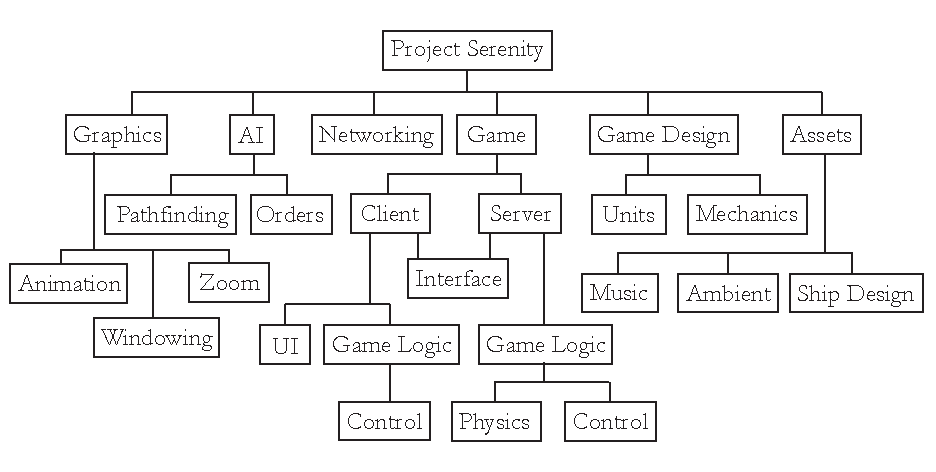
\includegraphics{res/wbs}
	\caption{Work Breakdown Structure of the game components.}
\end{figure*}

From the WBS we can further break the project down into components which are suited for weekly development cycles.

Term 2 releases will include a UI, an AI system and further improvements to the components as required. Assets such as music and additional ship designs are non-essential and will likely follow in a later release.

\begin{figure*}
	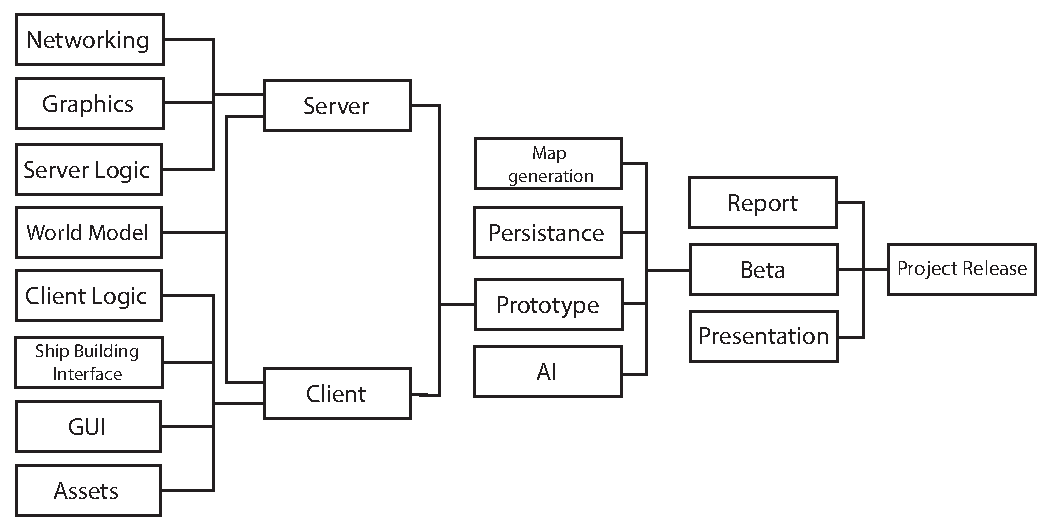
\includegraphics{res/dependency_tree}
	\caption[][-4.3em]{Component Dependency Graph.}
\end{figure*}

\begin{figure*}[h!]
	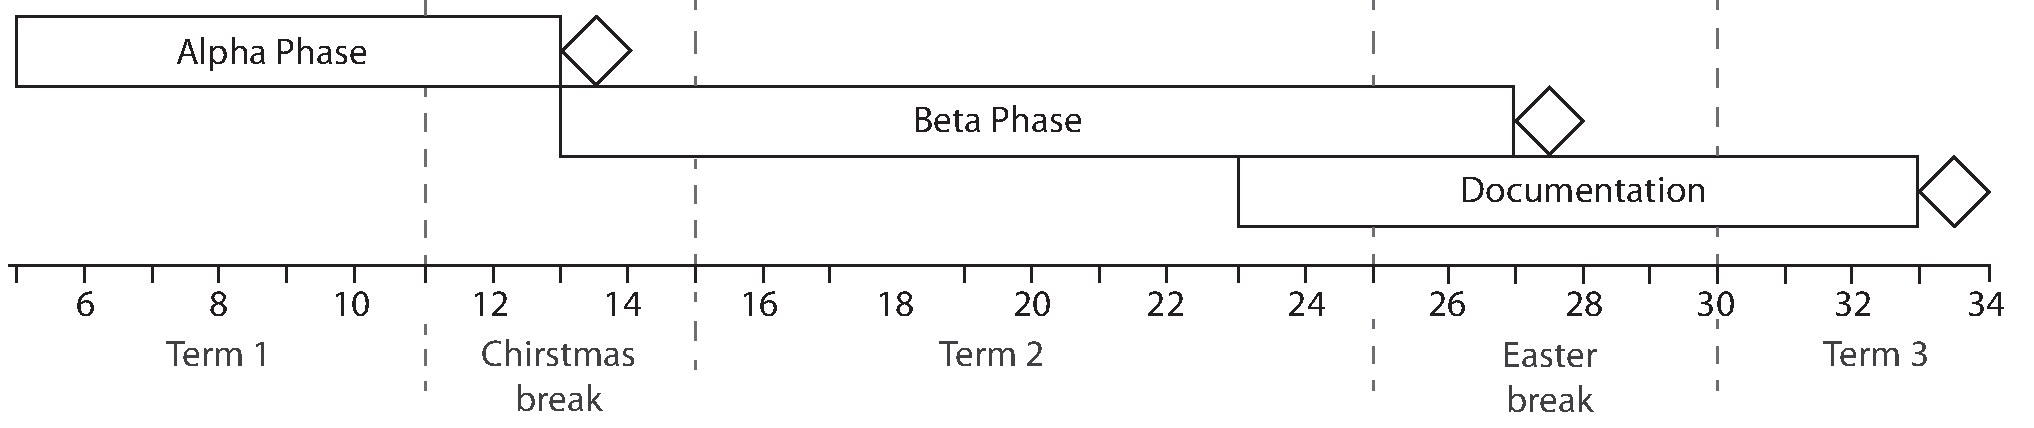
\includegraphics{res/gantt_chart_annotated}
	\caption{Phase level Gantt chart.}
\end{figure*}

The dependency tree shows which components are directly dependant on others, and show how delays will propagate through the project. The project dependency diagram shows that potential loss is minimised after a prototype is complete, that is to say there are fewer critical dependancies from the prototype level onwards. This information emphasises the priority of the server and client components should the project schedule require revising at a later stage.





\begin{figure}
	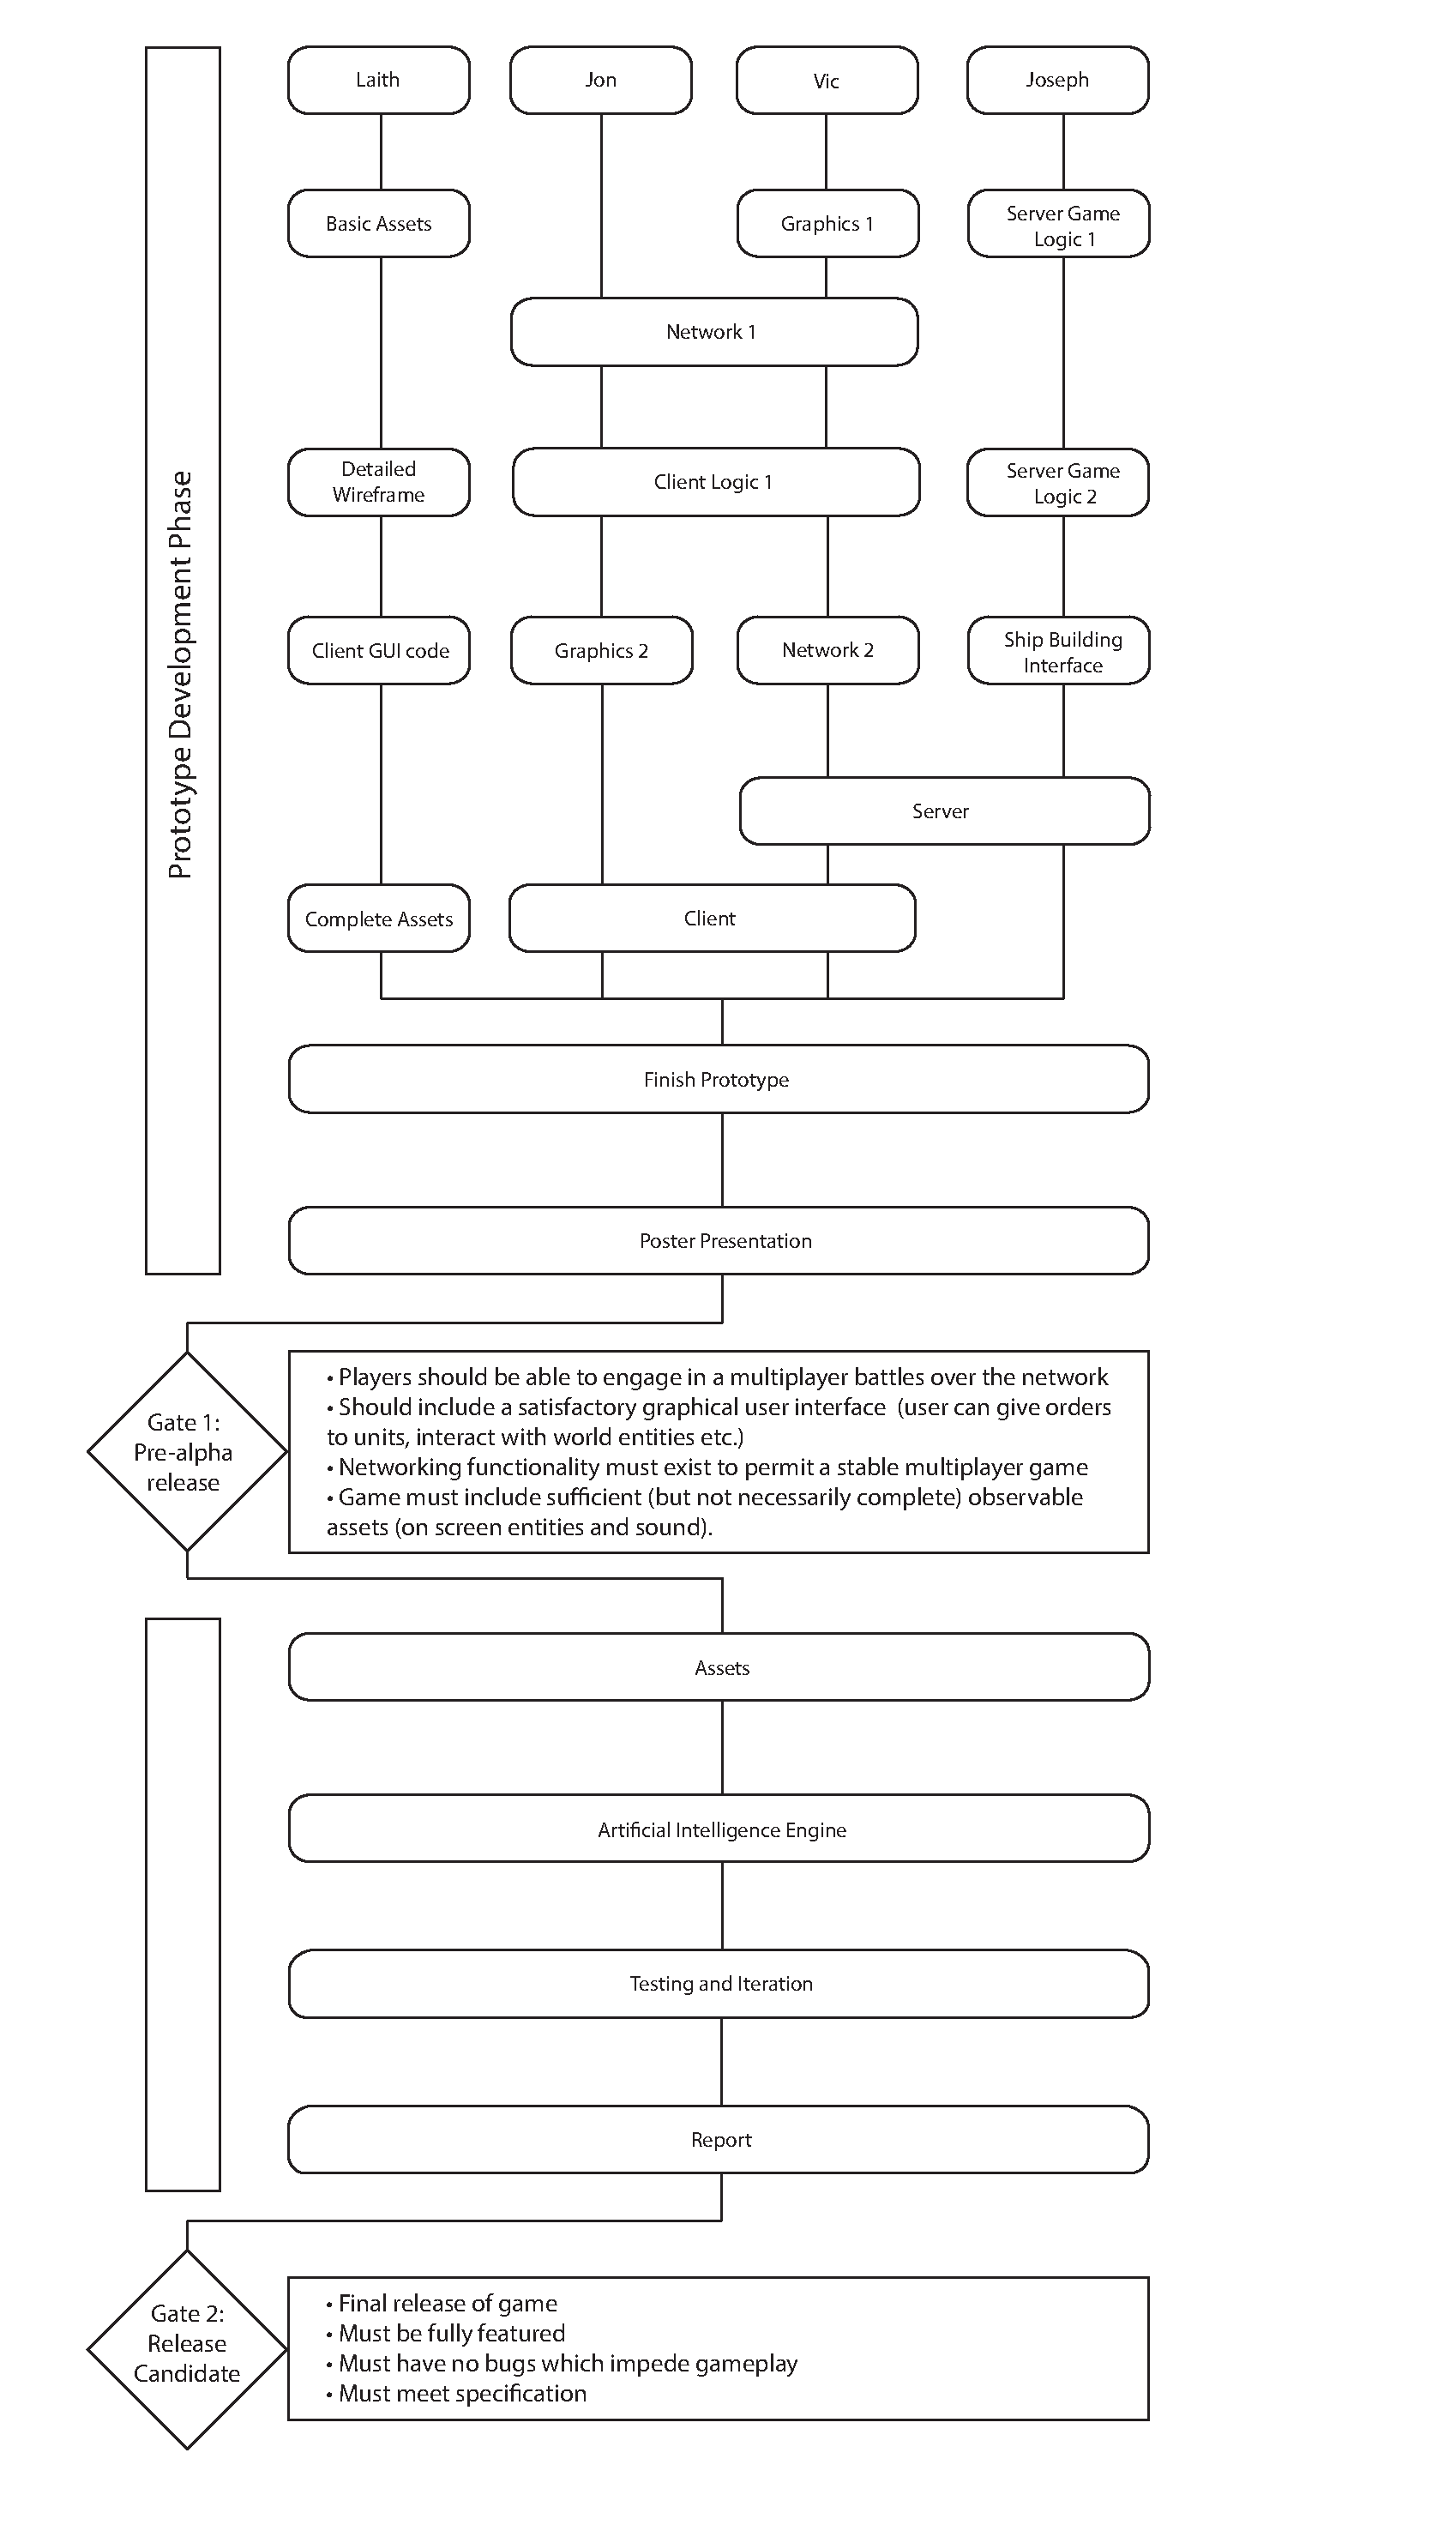
\includegraphics{res/stage_gate_diagram}
	\caption{Stage-gate model of work breakdown structure showing the division of labour across the various project phases. 
	The alpha phase is more thoroughly planned so we are able to see a weekly breakdown of tasks in the near future. The gates are project milestones, each of which details the requirements for proceeding through that gate into the next phase.}
\end{figure}

